\documentclass[aspectratio=169, 10pt]{beamer}

% --- Thème et couleurs ---
\usetheme{Madrid}
\usecolortheme{default}
\usepackage{tikz}
\usetikzlibrary{positioning, shapes.geometric, arrows.meta, calc}
\usepackage{graphicx}
\usepackage{float}
\usepackage{subcaption}
\usepackage[utf8]{inputenc}
\usepackage[T1]{fontenc}
\usepackage[french]{babel}
\usepackage{csquotes}
\usepackage{lmodern}
\usepackage{microtype}
\usepackage{amsmath, amssymb}
\usepackage{booktabs}
\usepackage{tabularx}
\usepackage{multirow}
\usepackage{colortbl}

% --- Couleurs ---
\definecolor{primary}{RGB}{0, 51, 102}
\definecolor{secondary}{RGB}{0, 102, 153}
\definecolor{accent}{RGB}{200, 50, 50}
\definecolor{successgreen}{RGB}{34, 139, 34}

% --- Personnalisation ---
\setbeamercolor{palette primary}{bg=primary, fg=white}
\setbeamercolor{palette secondary}{bg=secondary, fg=white}
\setbeamercolor{frametitle}{bg=primary, fg=white}
\setbeamercolor{title}{bg=primary, fg=white}
\setbeamercolor{block title}{bg=primary, fg=white}
\setbeamercolor{block body}{bg=primary!8, fg=black}
\setbeamertemplate{navigation symbols}{}

% --- Métadonnées ---
\title{Plateforme gouvernementale pour la cartographie des besoins des entreprises}
\subtitle{Présentation de l'état d'avancement}
\author{NDZESSA AVELE Bruno Landry}
\institute{ENSPM — Université de Maroua}
\date{Année académique 2025 / 2026}

\begin{document}
	
	% --- Page de titre ---
	\begin{frame}[plain]
		\titlepage
	\end{frame}
	
	% --- Plan ---
	\begin{frame}{Plan de la présentation}
		\tableofcontents[hideallsubsections]
	\end{frame}
	
	% --- Contexte ---
	\section{Contexte et problématique}
	\begin{frame}{Cadre institutionnel}
		\begin{block}{Structure d'accueil}
			\begin{itemize}
				\item MINEPAT
				\item DAPE (Division des Analyses et Politiques Économiques)
				\item DGEPIP
			\end{itemize}
		\end{block}
	\end{frame}
	
	\begin{frame}{Problématique}
		\begin{exampleblock}{Question centrale}
			Comment exploiter les données issues de l’enquête pour dynamiser le secteur privé moteur de la croissance économique ?
		\end{exampleblock}
	\end{frame}
	
	% --- Sources de données ---
	\section{Sources de données}
	\begin{frame}{Source des données : enquête MINEPAT 2025}
		\begin{itemize}
			\item Enquête nationale sur les besoins des entreprises
			\item Données stockées en MySQL (tables : identifications, besoins)
			\item Variables : raison sociale, région, taille, statut, secteur, date de début
			\item Besoins : financement, équipements, transport, emballages, innovation, etc.
		\end{itemize}
	\end{frame}
	
	% --- Résultats descriptifs ---
	\section{Analyse descriptive}
	\begin{frame}{Répartition des entreprises}
		\begin{figure}
			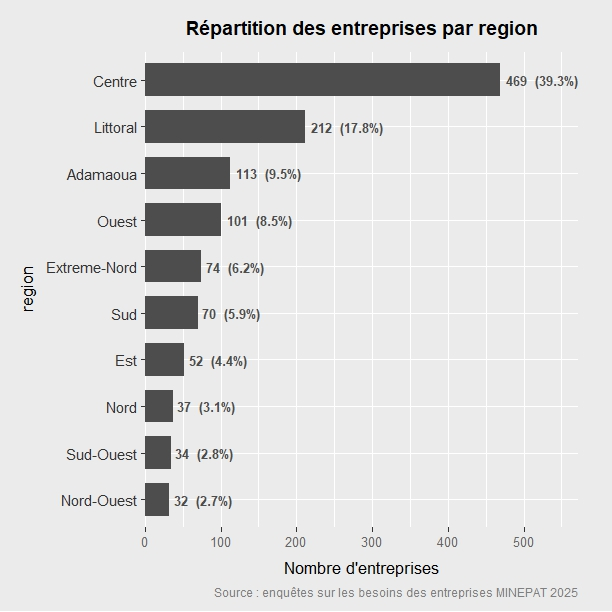
\includegraphics[width=0.7\textwidth]{repartition_region.jpeg}
			\caption{Répartition des entreprises par région}
		\end{figure}
	\end{frame}
	
	\begin{frame}{Répartition des besoins}
		\begin{figure}
			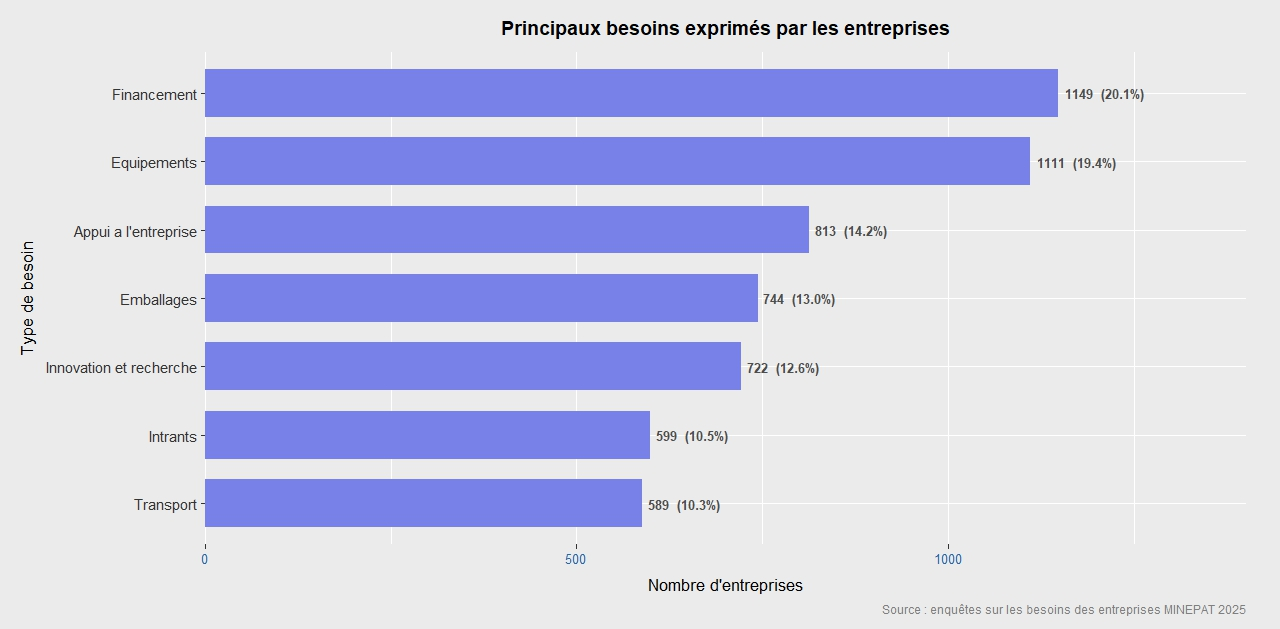
\includegraphics[width=0.7\textwidth]{repartition_besoins.jpeg}
			\caption{Répartition des besoins exprimés}
		\end{figure}
		\begin{alertblock}{Résultat clé}
			62,6\% des entreprises évoluent dans l’agroalimentaire. Les besoins dominants sont le financement (20,1\%) et les équipements (19,4\%).
		\end{alertblock}
	\end{frame}
	
	% --- Analyse bivariée ---
	\begin{frame}{Synthèse de l'analyse bivariée}
		\scriptsize
		\begin{tabular}{l|ccccc}
			\toprule
			Besoins & Statut & Région & Ancienneté & Secteur & Taille \\
			\midrule
			Intrants & 0,11 & 0,16 & Non & 0,29 & Non \\
			Financement & Non & Non & Non & 0,17 & Non \\
			Emballages & 0,19 & 0,13 & Non & \textbf{0,51} & Non \\
			Transport & 0,21 & 0,16 & Non & 0,35 & Non \\
			Équipements & 0,23 & 0,15 & 0,11 & \textbf{0,45} & Non \\
			Innovation & 0,26 & 0,14 & 0,13 & 0,37 & Non \\
			\bottomrule
		\end{tabular}
	\end{frame}
	
	% --- Analyse multidimensionnelle ---
	\section{Analyse multidimensionnelle}
	\begin{frame}{Pipeline méthodologique}
		\begin{itemize}
			\item ACM : réduction de dimension
			\item CAH : classification en 3 classes
			\item AFD : validation et prédiction
			\item Plateforme : recommandations ciblées
		\end{itemize}
	\end{frame}
	
	\begin{frame}{Projection ACM}
		\begin{figure}
			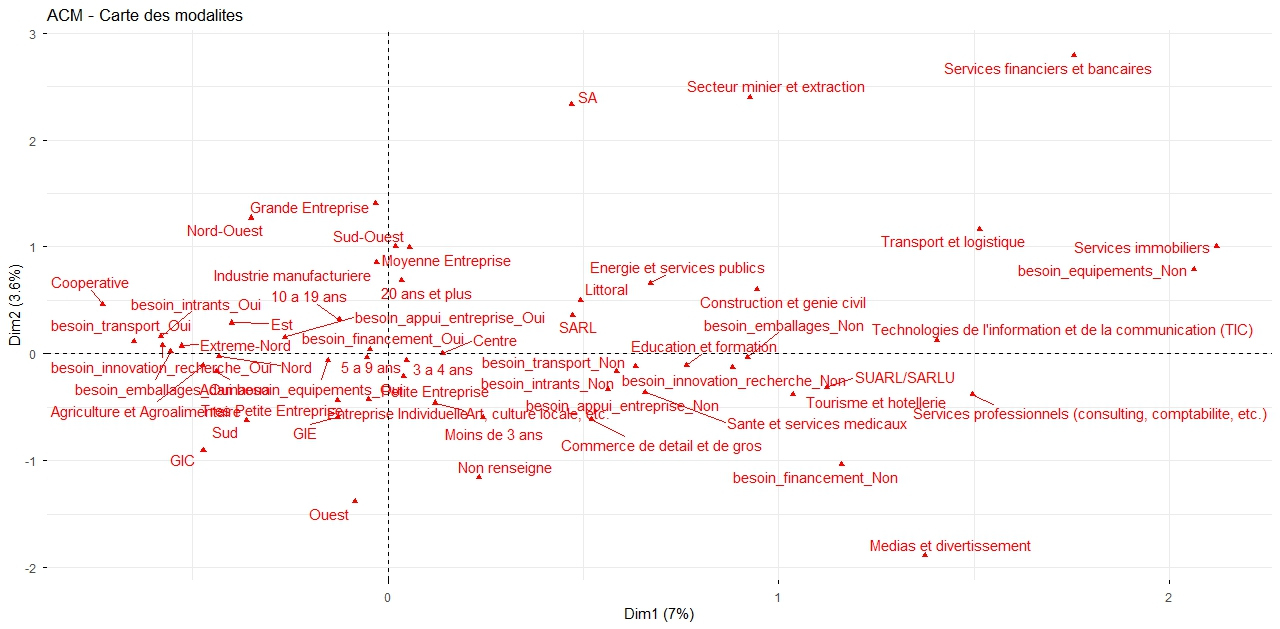
\includegraphics[width=0.7\textwidth]{projectionDesCategories.jpeg}
			\caption{Projection des modalités sur les axes 1 et 2}
		\end{figure}
	\end{frame}
	
	\begin{frame}{CAH : Dendrogramme}
		\begin{figure}
			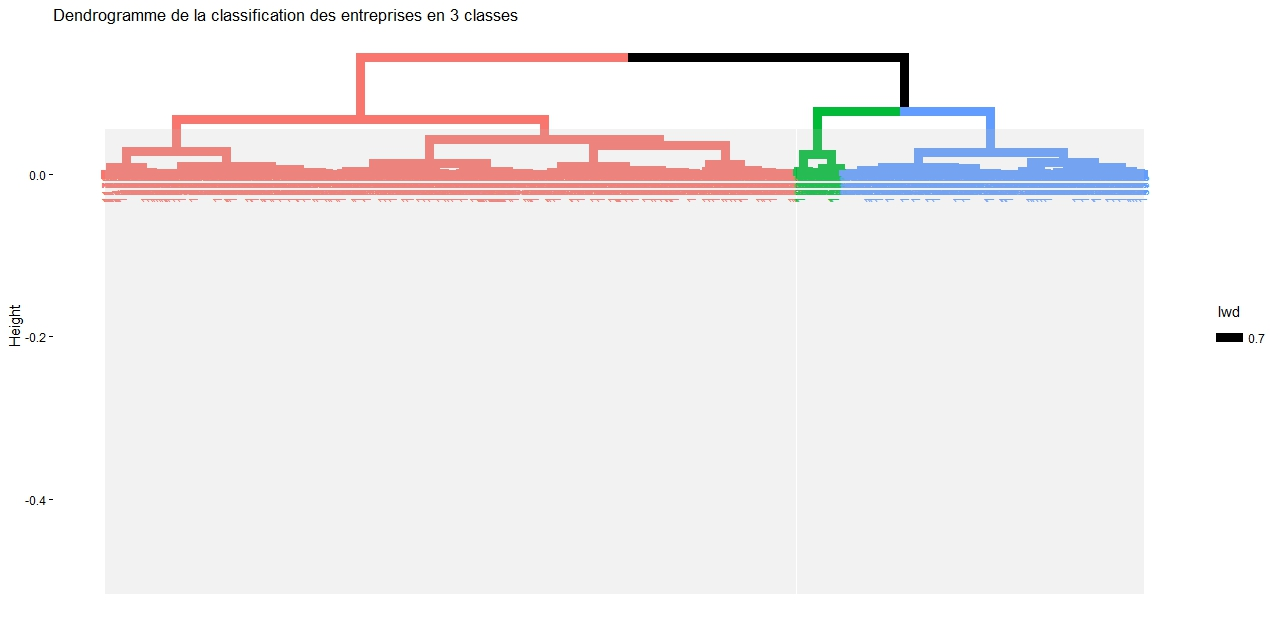
\includegraphics[width=0.7\textwidth]{dendrogramme.jpeg}
			\caption{Classification ascendante hiérarchique (Ward)}
		\end{figure}
	\end{frame}
	
\end{document}
